% !TEX program = xelatex
% Clean CV template — Letter (8.5×11in) — requires XeLaTeX
% -------------------------------------------------------------
\documentclass[10pt,letterpaper]{article}

% ---------- FONTS ---------------------------------------------
\usepackage{fontspec}
\IfFontExistsTF{Roboto}
    {\setmainfont{Roboto}}
    {\IfFontExistsTF{Helvetica Neue}
        {\setmainfont{Helvetica Neue}}
        {\setmainfont{Latin Modern Sans}}}

% ---------- GEOMETRY ------------------------------------------
\usepackage[
  letterpaper,
  left=0.55in, right=0.55in,
  top=0.8in,  bottom=0.8in
]{geometry}

% ---------- COLOURS & GRAPHICS --------------------------------
\usepackage[dvipsnames,svgnames,x11names]{xcolor}
\definecolor{primary}{HTML}{004A99}
\definecolor{accent}{HTML}{E6F4FF}

\usepackage{graphicx}
\usepackage{tikz}
\usetikzlibrary{calc}

% ---------- LAYOUT HELPERS ------------------------------------
\usepackage{paracol}
\columnratio{0.32}
\setlength{\columnsep}{0.25in}

\usepackage[most]{tcolorbox}
\tcbset{colback=accent, colframe=accent, boxrule=0pt, sharp corners}

\usepackage{enumitem}
\setlist[itemize]{noitemsep,topsep=0pt,leftmargin=*}

\usepackage{sectsty}
\allsectionsfont{\color{primary}\bfseries\uppercase}
\subsectionfont{\color{primary}\bfseries}
\renewcommand{\thesection}{}

\usepackage[hidelinks]{hyperref}

% ---------- UTILITIES -----------------------------------------
\newcommand{\cvName}[1]{\vspace*{0.3in}\textbf{\LARGE #1}}
\newcommand{\cvHeadline}[1]{\par\smallskip\textit{#1}}
\newcommand{\cvHr}{\vspace{0.5\baselineskip}\hrule height 1pt\color{primary}\vspace{0.7\baselineskip}}

% ==============================================================
\begin{document}\small
\begin{paracol}{2}

% ================== SIDEBAR ====================================
\begin{leftcolumn}
\begin{center}
\begin{tikzpicture}
  \node[draw=primary,line width=1pt,circle,inner sep=0pt,minimum width=1.6in]  {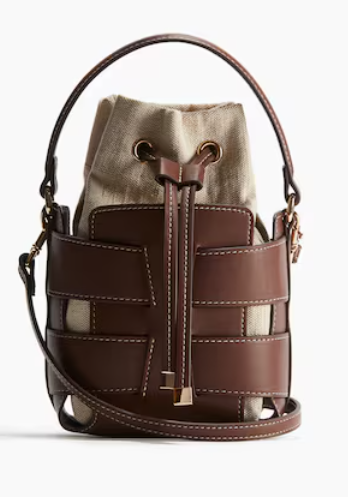
\includegraphics[width=1.6in,height=1.6in]{a431e42195d2405b962d33a34a39df86.png}};
\end{tikzpicture}
\end{center}

\vspace{0.6in}

\cvName{Pape FALL}
\cvHeadline{Data Scientist}
\cvHr

\section*{Contact}
0753481453\\
\href{mailto:jean@prepaya.fr}{jean@prepaya.fr}\\
\href{https://www.linkedin.com/in/pape-saliou-fall-43154a211}{linkedin.com/in/pape-saliou-fall-43154a211}\\
Paris, France

\cvHr
\section*{Languages}
French (Native)\\
English (Fluent)

\cvHr
\section*{Key Skills}
Python\\
Machine Learning\\
SQL\\
Data Visualization (Power BI, Tableau)

\cvHr
\section*{Hobbies}
Reading tech blogs\\
Playing chess\\
Hiking
\end{leftcolumn}

% ================== MAIN COLUMN ================================
\begin{rightcolumn}
\section*{Professional Summary}
Data Scientist with strong background in machine learning, statistical modeling and data visualization. Experienced in transforming complex datasets into actionable insights to drive strategic decision-making. Passionate about leveraging data to solve real-world problems and deliver measurable business value.

\vspace{0.4in}
\section*{Work Experience}

\begin{tcolorbox}
  \begin{minipage}[t]{0.48\linewidth}
    Jan 2022\\
    \textbf{Prepaya — Paris, France}\\
    \begin{itemize}
      \item Developed predictive models to forecast customer churn, improving retention by 12\%.
      \item Automated data pipelines in Python, reducing reporting time by 40\%.
      \item Collaborated with cross-functional teams to define KPIs and build interactive dashboards.
    \end{itemize}
  \end{minipage}\hfill
  \begin{minipage}[t]{0.48\linewidth}\raggedleft
    Dec 2023
  \end{minipage}
\end{tcolorbox}

\vspace{0.5in}
\section*{Education}
\begin{tcolorbox}[colback=white,boxrule=1pt,colframe=primary]
  Master 2 Data Science\\
  Sorbonne Université\\
  2012 – 2015
\end{tcolorbox}

\section*{Certifications}
\begin{itemize}
  \item ksLD — KSLQKBC (Jul-2024)
\end{itemize}

\end{rightcolumn}
\end{paracol}
\end{document}